\chapter{Implementace hardwarových komponent}

\section{Sběrnice/Jádro emulátoru}

Sběrnice představuje do jisté míry nervový systém celého emulátoru, neboť nejen propojuje hlavní 
hardwarové komponenty, ale musí se také starat o jejich paměťovou správu. 
Díky tomuto faktoru sběrnice v emulátoru vytváří všechny komponenty a řeší jejich vzájemné závislosti, čímž
vytváří pomyslné jádro emulátoru.

Jelikož komponenty mohou být vzájemně sdíleny, bylo nutné zvolit vhodnou 
strukturu pro správu jednotlivých objektů. Pro tyto účely jsem se rozhodl použít \textit{shared\_ptr} ze 
standardní knihovny \textit{C++}. Nejenže bude paměť spravována automaticky, ale lze velice jednoduše vytvořit duplicitní reference na tentýž objekt, viz obrázek \ref{bus-ownage}.

\begin{figure}[hbt]
    \centering
    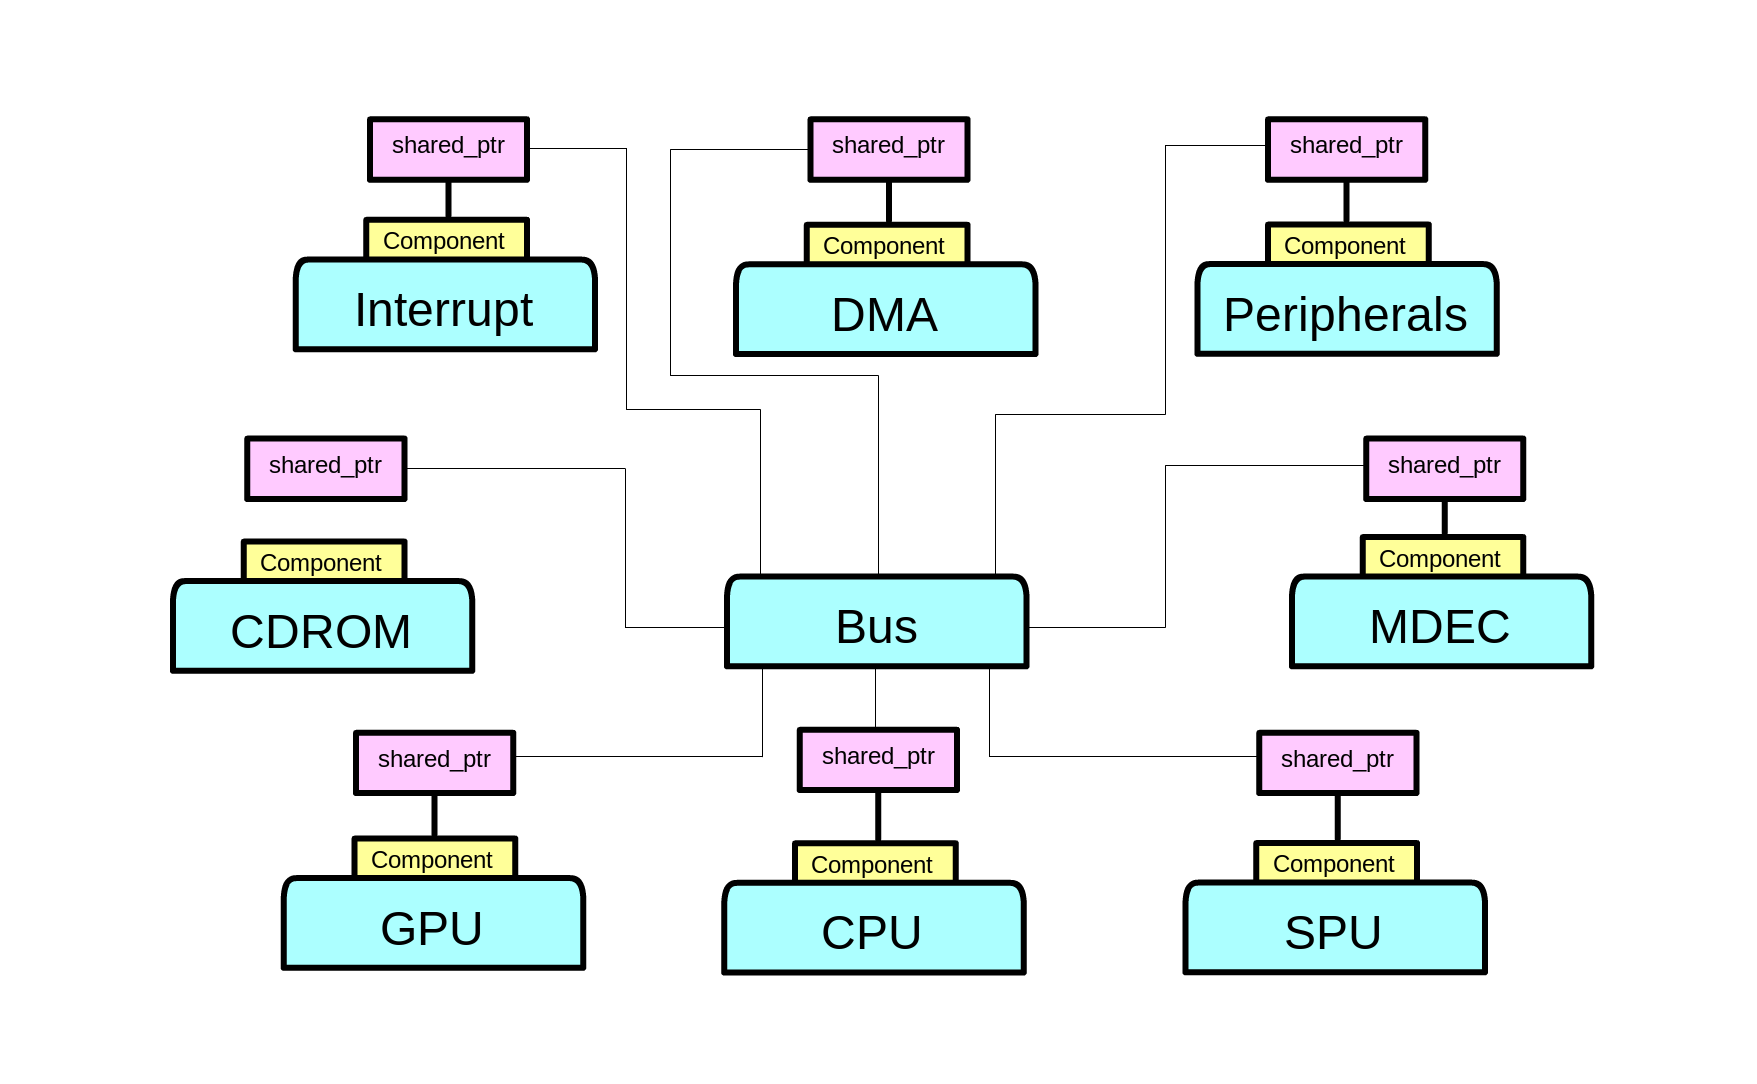
\includegraphics[width=0.8\textwidth]{obrazky-figures/bus-ownage.png}
    \caption[Návrh sběrnice]{Sběrnice pomocí \textit{shared\_ptr} struktury může vlastnit jednotlivé komponenty, ale také umožňuje sdílení mezi těmito komponentami.}
    \label{bus-ownage}
\end{figure}

Další odpovědností sběrnice je správná distribuce čtení a zápisů jednotlivým komponentám. 
Všechny tyto paměťové operace závisejí na \textit{Memory-mapped I/O}. \textit{Memory-mapped I/O} mapuje 
lineární 32-bitový paměťový prostor na segmenty, skrz které může sběrnice ovládat jednotlivé komponenty\footnote{Paměťová mapa PlayStation \cite{PSXSpec}: \url{https://psx-spx.consoledev.net/iomap/}}.
Jakákoliv komponenta v emulátoru může zavolat 2 funkce sběrnice pro interakci s ostatními komponentami: \textit{dispatch\_read} a \textit{dispatch\_write}.
Obě funkce na základě šířky dat a paměťové mapy popsané v tabulce \ref{memory-map} rozhodnou, které komponentě tato data zaslat, či ze které komponenty data získat.

\begin{table}[htbp]
    \caption{Paměťová mapa}
    \begin{center}
    \begin{tabular}{ |c|c|r| }
    \hline
    \textbf{Název} & \textbf{Lokace} & \textbf{Velikost} \\
    \hline
    RAM & 0x00000000 & 2 MiB + 3x mirrors \\
    Expansion & 0x1F000000 & 1 MiB \\
    Scratchpad & 0x1F800000 & 1 KiB \\
    Ovladač paměti & 0x1F801000 & 36 B \\
    Periférie & 0x1F801040 & 16 B \\
    Serial & 0x1F801050 & 16 B \\
    Ovladač RAM & 0x1F801060 & 4 B \\
    Ovladač přerušení & 0x1F801070 & 8 B \\
    DMA & 0x1F801080 & 128 B \\
    DotClock Časovač & 0x1F801100 & 16 B \\
    HBlank Časovač & 0x1F801110 & 16 B \\
    SystemClock/8 Časovač & 0x1F801120 & 16 B \\
    CDROM & 0x1F801800 & 4 B \\
    GPU & 0x1F801810 & 8 B \\
    MDEC & 0x1F801820 & 8 B \\
    SPU & 0x1F801C00 & 1 KiB \\
    I/O porty & 0x1F802000 & 8 KiB \\
    BIOS & 0x1FC00000 & 512 KiB \\
    Ovladač cache & 0x1FFE0130 & 4 B \\
    \hline
    \end{tabular}
    \end{center}
    \label{memory-map}
\end{table}

V systému je několik paměťových regionů, které slouží pro ukládání generických dat. Jsou to: \textit{RAM}, \textit{Expansion}, \textit{Scratchpad (nebo taky známá jako fast RAM, či data cache)}, \textit{Video RAM} (vlastněno \textit{GPU}) a \textit{Sound RAM} (vlastněno \textit{SPU}). K těmto paměťovým regionům lze přistupovat s různou šířkou dat (8, 16 a 32 bitové jednotky). Pomocí \textit{STL} knihovny \textit{C++} byla implementována třída \textit{MemoryRegion}, pomocí níž jsou všechny tyto emulované paměťové regiony realizovány. Třída řeší správné adresování na základě různé datové šířky a také zajišťuje korektní kontroly mezí.

Ačkoliv standardní knihovna \textit{C++} má způsob, jak spravovat statické pole pomocí třídy \textit{array}, ošetření přístupů k tomuto poli s různými datovými šířkami by vyžadovalo extrahování ukazatele na alokované pole pomocí funkce \textit{array::data}, čímž bychom ztratili kontrolu mezí, protože třída \textit{array} vyžaduje specifikaci typu uložené jednotky. Proto bylo nutné implementovat zvláštní třídu pro tyto speciální účely.

Jelikož sběrnice má 32-bitovou šířku, mohlo by se zdát, že stačí pouze na základě paměťové mapy vzít danou 
adresu a rozdistribuovat ji příslušné komponentě. Nicméně sběrnice tohoto systému má 2 zvláštnosti: 
Správa virtuální paměti popsané v sekci [\ref{virtual-mem}] a přímý zápis do vyrovnávací paměti instrukcí popsané v sekci [\ref{icache-direct}].

\subsection{Virtuální paměť} \label{virtual-mem}

Jak bylo naznačeno, \textit{PlayStation} je do jisté míry zjednodušená verze 
stolního počítače a existují určité artefakty a ostatky, které zajišťovaly plnou funkčnost stolního počítače. 
Jedním z takovýchto artefaktů je virtuální paměť. I přesto, že procesor má 
podporu \textit{Translation Lookaside Bufferu (TLB)} pro efektivní správu virtuální paměti, \textit{PlayStation} jej vůbec nevyužívá a všechny přístupy do paměti jsou v zásadě absolutní.
To, co zůstalo z virtualizace paměti, je maskování všech adres, které přijdou na sběrnici a na základě velikosti zapisovaných či čtených dat probíhá maskování odlišně.
Nejdříve se u každého přístupu zahodí vrchní 3 bity. 
Poté u půl-slova (16 bitů) se zahodí spodní 1 bit a u slova (32 bitů) se zahodí spodní 2 bity. 
Zahození spodních bitů souvisí se zarovnáním do paměti\footnote{Přístup do paměti \cite{PSXSpec}: \url{https://psx-spx.consoledev.net/memorymap/}}.

\subsection{Vyrovnávací paměť instrukcí} \label{icache-direct}

Druhá zvláštnost, na kterou je třeba myslet při distribuci čtení a zápisu, je vyrovnávací paměť instrukcí uvnitř \textit{CPU}. 
Tato vyrovnávací paměť slouží pro rychlé získávání instrukcí z hlavní paměti a teoreticky by nikdy 
neměla nastat situace, kdy ve vyrovnávací paměti bude něco jiného, než co je obsaženo v hlavní paměti. 
Ovšem to není u tohoto systému vždy pravda.

\textit{CPU} má speciální stav, který se dá programově nastavit a který takzvaně \textit{izoluje vyrovnávací paměť instrukcí}. 
Pokud se  \textit{CPU} nachází v tomto stavu, pak každé čtení za účelem získat instrukce (\textit{fetch} fáze  \textit{CPU}) nikdy nebude přecházet do hlavní paměti, ale do této vyrovnávací paměti a \textbf{každý} zápis bude modifikovat vyrovnávací paměť namísto hlavní paměti.
\textit{CPU} tedy jinými slovy poskytuje přímý přístup do této vyrovnávací paměti.
Pokud toto není správně ošetřeno a simulováno, \textit{PlayStation} nebude schopen nastartovat\footnote{Koprocesor 0, registr 12, bit 16 \cite{PSXSpec}: \url{https://psx-spx.consoledev.net/cpuspecifications/\#cop0r12-sr-system-status-register-rw}}, 
protože \textit{BIOS} se v prvé řadě snaží vyčistit tuto vyrovnávací paměť tak, že ji vyplní samými nulami. Nicméně
pokud zápisy nejsou filtrovány, \textit{BIOS} přepíše nulami svůj vlastní \textit{shell} program a tedy zničí svoji zaváděcí fázi.

Toto chování je reflektováno ve funkci \textit{dispatch\_write} uvnitř sběrnicového modulu \textit{Bus}, kde se kontroluje stav \textit{CPU} a filtrují se zápisy.

\subsection{Časování}

Každá hardwarová komponenta pracuje v reálném čase paralelně a nezávisle. Situaci dále zhoršuje fakt, že každá komponenta má odlišnou frekvenci hodin\footnote{Časování \cite{PSXSpec}: \url{https://psx-spx.consoledev.net/timers/}, \url{https://psx-spx.consoledev.net/graphicsprocessingunitgpu/\#gpu-timings}}:

\begin{itemize}
    \label{Rychlost hodin komponent}
    \item{\textbf{CPU} - 33.868800 MHz}
    \item{\textbf{GPU} - 53.222400 MHz}
    \item{\textbf{SPU} - 44.100 KHz}
    \item{\textbf{DotClock Timer} - 4.980705 MHz (Průměr)}
    \item{\textbf{HBlank Timer} - 9923 Hz (NTSC), 9943 Hz (PAL)}
    \item{\textbf{System Clock/8 Timer} - 4.233600 MHz}
\end{itemize}

Tento problém je řešen tak, že emulátor simuluje každou komponentu sekvenčně a zvlášť v malých kvantech. 
Množství hodinových cyklů alokovaných pro danou komponentu reflektuje předchozí list hodnot. 
Tento přístup ovšem může způsobit časovou dilataci mezi jednotlivými komponentami a vést k narušení jejich synchronizace. 
Při volbě časového kvanta ho nesmíme zvolit příliš malé, protože by došlo k nesprávnému zaokrouhlení na základě časovací tabulky a nepřesnost časování by byla větší. 
Zároveň však kvantum nesmíme zvolit příliš velké, protože by se komponenty nemusely dostat včas ke slovu. 
Dvě komponenty, pro které je synchronizace nejdůležitější, jsou \textit{CPU} a \textit{GPU}. 
Protože je \textit{GPU} o $\frac{11}{7}$ rychlejší, zvolil jsem tedy časovou konstantu $105$. Výsledek formule $105\times\frac{11}{7}=165$ je celé číslo a není
tedy potřeba řešit zlomkovou část časování.

\subsection{Načítání her/programů}

Při inicializaci jádra emulátoru musí uživatelské rozhraní specifikovat cestu k obrazu disku hry,
nebo cestu k \textit{PSX Executable} souboru. V obou případech se musí upravit vnitřní stav
emulátoru, aby byl schopen dodaný program spustit.

U \textbf{načítání disku} jádro přijímá speciální formát souboru obsahující nejenom data hry, ale také sub-kanály.
Odkaz na obraz hry (Obsah není přečten, pouze se otevře soubor ve čtecím módu) je předán
\textit{CD-ROM}, která hru analyzuje a rozdělí ji do stop (tento emulátor nepodporuje více stop v jedné hře, jako jsou například audio stopy, čili \textit{CD-ROM} vytvoří pouze jednu stopu).
Poté je při vyžádání dat z \textit{CD-ROM} mechaniky soubor v určitém místě přečten jako 2352-bytový sektor.

\begin{table}[htbp]
    \caption{Formát PSX Executable}
    \begin{center}
    \begin{tabular}{ |c|l|r| }
     \hline
     \textbf{Název} & \textbf{Typ} & \textbf{Velikost} \\
     \hline
     PSX magic & uint8 & 8 \\
     Výplň/Neznámé & uint8 & 8 \\
     Program Counter & uint32le & 1 \\
     Global Pointer (R28) & uint32le & 1 \\
     Pozice \textit{TEXT} Sekce & uint32le & 1 \\
     Velikost \textit{TEXT} Sekce & uint32le & 1 \\
     Pozice \textit{DATA} Sekce & uint32le & 1 \\
     Velikost \textit{DATA} Sekce & uint32le & 1 \\
     Pozice \textit{BSS} Sekce & uint32le & 1 \\
     Velikost \textit{BSS} Sekce & uint32le & 1 \\
     Stack Pointer Base & uint32le & 1 \\
     Stack Pointer Offset & uint32le & 1 \\
     Výplň/Neznámé & uint8 & 20 \\
     Sony Podpis & uint8 & 1972 \\
     \textit{TEXT} Sekce & uint32le & ... \\
     \textit{DATA} Sekce & uint32le & ... \\
     \textit{BSS} Sekce & uint32le & ... \\
     \hline
    \end{tabular}
    \end{center}
    \label{psx-executable-format}
\end{table}

Při načítání \textbf{PSX Executable} musí jádro nejdříve zpracovat hlavičku spustitelného souboru. Obsah této hlavičky je popsán v tabulce \ref{psx-executable-format}\footnote{formát PSX executable \cite{PSXSpec}: \url{https://psx-spx.consoledev.net/cdromfileformats/\#filenameexe-general-purpose-executable}}.
Z ní jádro extrahuje počáteční hodnoty \textit{CPU} registrů a vyplní \textit{RAM} paměť instrukcemi programu v \textit{TEXT} Sekci.
Aby se program správně spustil, musí se nejdřív provést inicializační rutina, kterou provádí \textit{BIOS}.
Jakmile \textit{BIOS} začne spouštět svůj \textit{shell}, je třeba \textit{CPU} ručně přerušit, nastavit registry na 
jejich iniciální hodnoty tak, jak jsou obsaženy v hlavičce \textit{PSX Executable},
přepsat \textit{RAM} paměť a posléze znovu povolit simulaci systému.
Pro tyto účely lze využít \textit{Breakpointy}, kde přerušíme chod systému, jakmile \textit{CPU} dosáhne adresy \textbf{0x8003'0000}, což
indikuje počátek \textit{shell} programu.

\section{Centrální procesorová jednotka (CPU)}

Pokud je sběrnice nervovým systémem, pak \textit{CPU} je mozkem \textit{PlayStation} systému. Jde
o \textit{MIPS R3000A} 32-bitový \textit{RISC} procesor. Jeho architektura je založena na \textit{MIPS I} redukované instrukční sadě.
\textit{CPU} má celkem 5 fází, ve kterých se může jedna instrukce nacházet a které CPU provádí paralelně v nepřetržité smyčce:

\begin{itemize}
    \item{\textbf{Fetch (IF)} fáze - získání následující instrukce z paměti \textit{RAM}.}
    \item{\textbf{Decode (ID)} fáze - dekódování instrukce a zjištění následující operace.}
    \item{\textbf{Execute (EX)} fáze - \textit{CPU} provede dekódovanou instrukci (aritmetickou či logickou operaci).}
    \item{\textbf{Memory Access (MEM)} fáze - pokud instrukce přistupuje do paměti, data jsou pomocí sběrnice přečtena či zapsána do paměti \textit{RAM}.}
    \item{\textbf{Write Back(WB)} fáze - Výsledek instrukce je zapsán do souboru registrů.}
\end{itemize}


Emulátor tuto linku částečně respektuje, ale neprovádí ji paralelně. \textbf{IF} fáze je
implementovaná jako samostatná jednotka, ovšem fáze \textbf{ID}, \textbf{EX}, \textbf{MEM} a \textbf{WB}
jsou prováděny naráz, přičemž u fází \textbf{MEM} a \textbf{WB} pak navíc je nutná režie pro
zpoždění načítaných a ukládaných hodnot pro simulaci paralelního zpracování jednotlivých fází. Tato režie je popsána níže v sekci [\ref{register-load-delay}].
Transformace toku instrukcí v emulátoru na funkční kód je prováděna pomocí jednoduché interpretace. Emulátor uchovává tabulku ukazatelů na funkce, přičemž operační kód instrukce pak specifikuje index do této tabulky ukazatelů, kde indexovaná funkce pak implementuje funkcionalitu dané instrukce.

\subsection{Vnitřní stav \textit{CPU}} \label{cpu-state}

Pro ukládání mezivýsledků a pro obecné zpracování logiky, \textit{CPU} obsahuje celkem \textbf{32} 32-bitových registrů, plus \textbf{2} 32-bitové registry, které
jsou specializované pro práci s násobícími a dělícími instrukcemi \cite{MIPSSpec}. 
\textit{Nultý} registr je speciální tím, že při čtení vrací vždy nulu a jakýkoliv zápis do něj je ignorován.

Vzhledem k tomu, že \textit{nultý} registr má speciální chování a navíc registry vykazují fenomén zpoždění načítání hodnot, viz sekci [\ref{register-load-delay}], bylo nutné vytvořit v emulátoru speciální logiku pro načítání hodnoty do registru. Tato funkcionalita je implementována ve funkci \textit{CPU::set\_register}. 

\subsection{Zpoždění načítání hodnot} \label{register-load-delay}

\textit{MIPS R3000A}, jako každý \textit{RISC} procesor, vykazuje zvláštní jev při načítání hodnot do registrů.
Pokud se snažíme načíst hodnotu z paměti \textit{RAM} do procesoru, zpoždění způsobené načítáním hodnoty má za následek
opožděné nastavení registru na přečtenou hodnotu o jeden procesorový takt \cite{MIPSSpec}. 
Toto je způsobeno samotným návrhem \textit{RISC} architektury a je nutné tuto situaci ošetřit. 

V emulátoru je tento fenomén simulován pomocí dvou registrových přihrádek, které fungují jako fronta.
Kdykoliv chce \textit{CPU} přečíst hodnotu z paměti \textit{RAM}, místo přímého nastavení registru,
přečtená hodnota spolu s indexem výsledného registru v prvním taktu je vložena do fronty a po druhém taktu se 
modifikuje registrové pole. V sekci [\ref{cpu-state}] bylo řečeno, že nultý registr při zápisu ignoruje hodnotu a při čtení vždy vrací hodnotu nula. Díky tomu lze prázdnou přihrádku reprezentovat jako zapisování do nultého registru.

Je nutné také pamatovat na situaci, kdy je ve frontě připravená hodnota, ale mezitím přijde jiná instrukce, 
která stejný registr modifikuje. V takovém případě je nutné frontu vyčistit, aby se výsledný registr neobsahoval špatnou hodnotu. Příklad opožděného načítání můžeme vidět v obrázku \ref{load-delay}.

\begin{figure}[hbt]
    \centering
    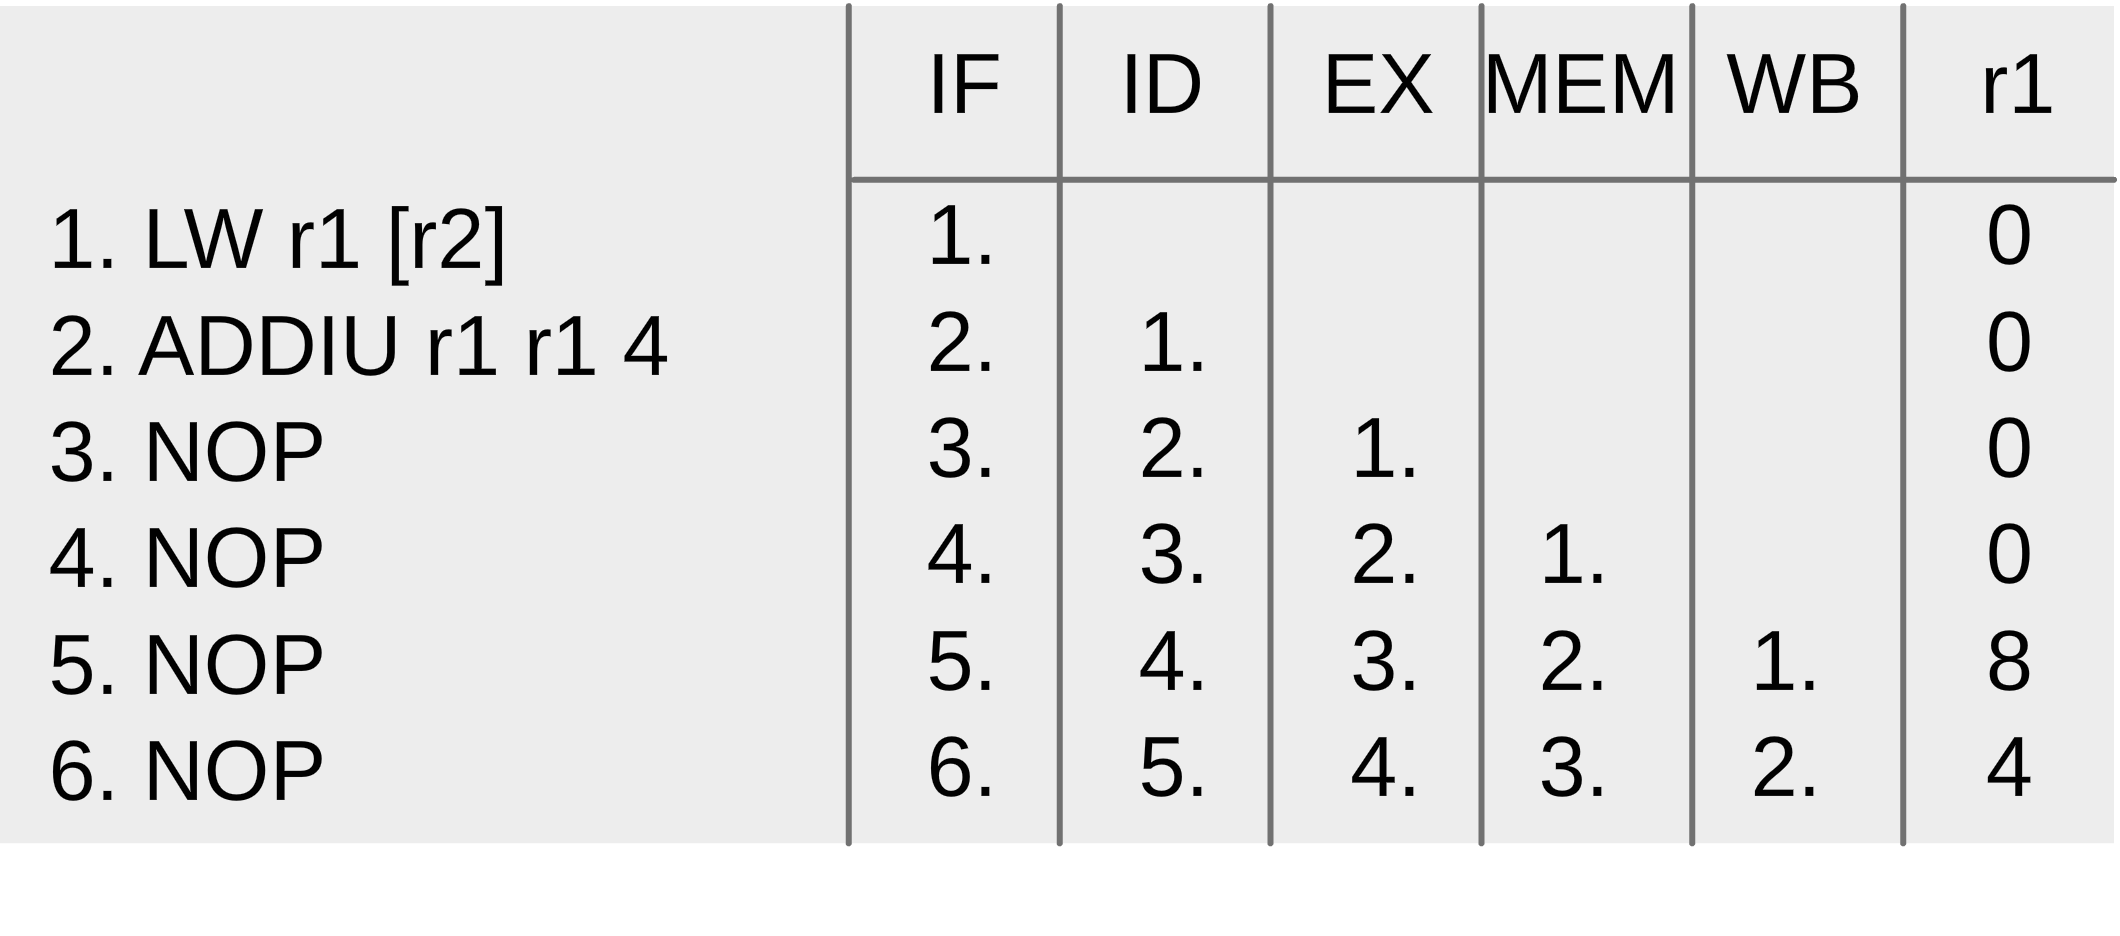
\includegraphics[width=0.8\textwidth]{obrazky-figures/load-delay.png}
    \caption[Opožděné načítání hodnot z paměti]{Příklad programu a vizualizace opoždění načtení hodnoty z paměti \textit{RAM}. Od toku programu bychom očekávali,
    že z adresy \textit{0} se přečte 32-bitová hodnota (dejme tomu hodnota \textit{8}) a poté se k ní přičte \textit{4}, přičemž ve výsledku
    v registru \textit{r1} by měla být výsledná hodnota \textit{12}. Protože je ovšem přečtení z paměti opožděno, \textit{ADDIU} instrukce
    počítá se špatnou hodnotou. Řešením by bylo vložit mezi instrukce \textit{1.} a \textit{2.} \textit{NOP}, nebo jinou užitečnou nezávislou instrukci.}
    \label{load-delay}
\end{figure}

\subsection{Zpoždění skoku}

Podobně jako opožděné načítání hodnot do registru, design 5-stupňové architektury má na svědomí ještě jeden problém.
Tento artefakt se vyskytuje u všech skokových instrukcí a má za následek že bez ohledu na to, zda-li se v případě 
podmíněných skokových instrukcí skočí nebo ne, následující instrukce po skokové instrukci se vždy provede \cite{MIPSSpec}.

To je způsobeno tím, že následující instrukce je již načtena a dekódována uvnitř \textit{CPU}. 
Kompilátory té doby byly dobře seznámeny s tímto fenoménem a ve většině případů vyplnily instrukci za skokem prázdnou instrukcí. 
Z tohoto důvodu je každý skok v emulátoru zpožděn o jeden takt.

\subsection{Zpracování breakpointů}

Pro snazší debugování při vývoji hry, \textit{CPU} podporovalo softwarové a hardwarové \textit{breakpointy}.
Jelikož breakpointy indikovaly buď špatný tok programu, či špatnou práci s hardwarovou komponentou,
v emulátoru je zpracování breakpointů dosti zjednodušené a nereflektuje jejich reálně zpracování, jak by je zpracoval původní systém. 
\textit{CPU} v emulátoru uchovává množinu adres pomocí třídy \textit{set} ze standardní knihovny \textit{C++}, kde pokud programový čítač narazí na některou z nich, celý emulátor je pozastaven a počká, až přijde potvrzení
breakpointu od jádra emulátoru. Breakpoint je posléze smazán z množiny adres a \textit{CPU}
pokračuje dále v provádění programu.

Breakpoint je v celém emulátoru využit pouze jednou a to při načítání \textit{PSX Executable} souboru.

\subsection{Instrukční sada}

\begin{figure}[hbt]
	\centering
	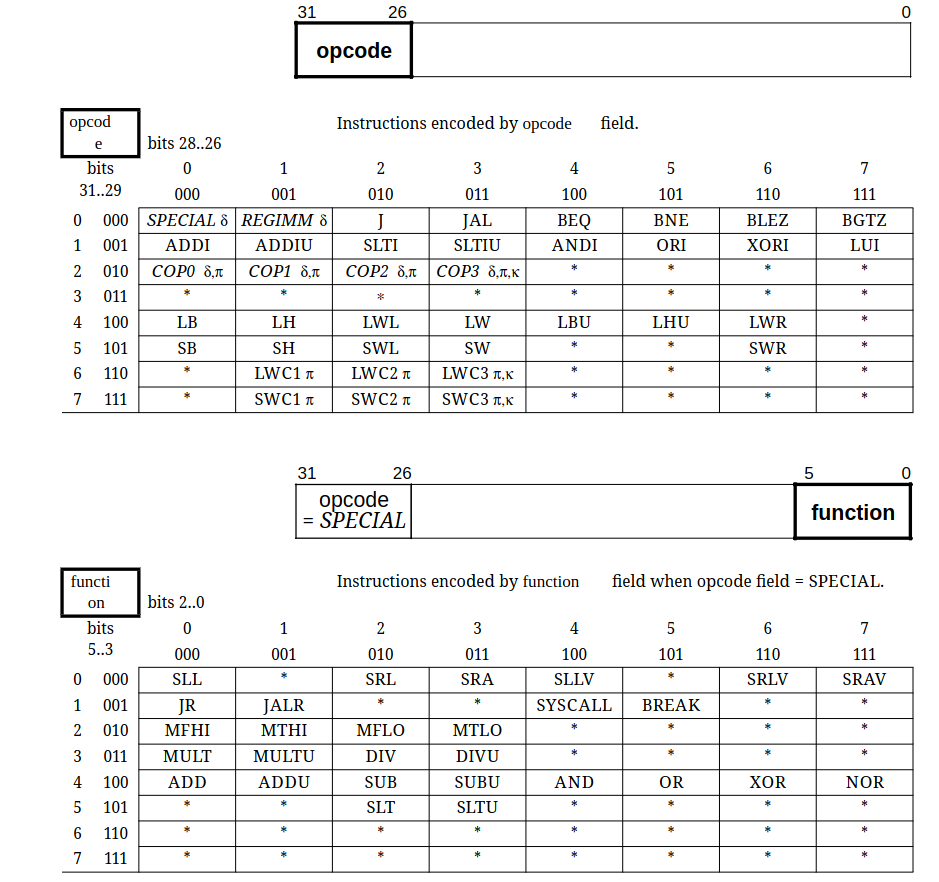
\includegraphics[width=0.8\textwidth]{obrazky-figures/instruction-map.png}
	\caption[\textit{MIPS I} instrukční sada]{Kompletní mapa všech \textbf{69} instrukcí podle \textit{MIPS} specifikace \cite{MIPSInsSpec}. V nespecifickém pořadí,
    procesor má instrukce pro ovládaní toku programu, aritmetické instrukce, logické instrukce a instrukce pracující s pamětí.}
	\label{instruction-map}
\end{figure}

\begin{figure}[hbt]
	\centering
	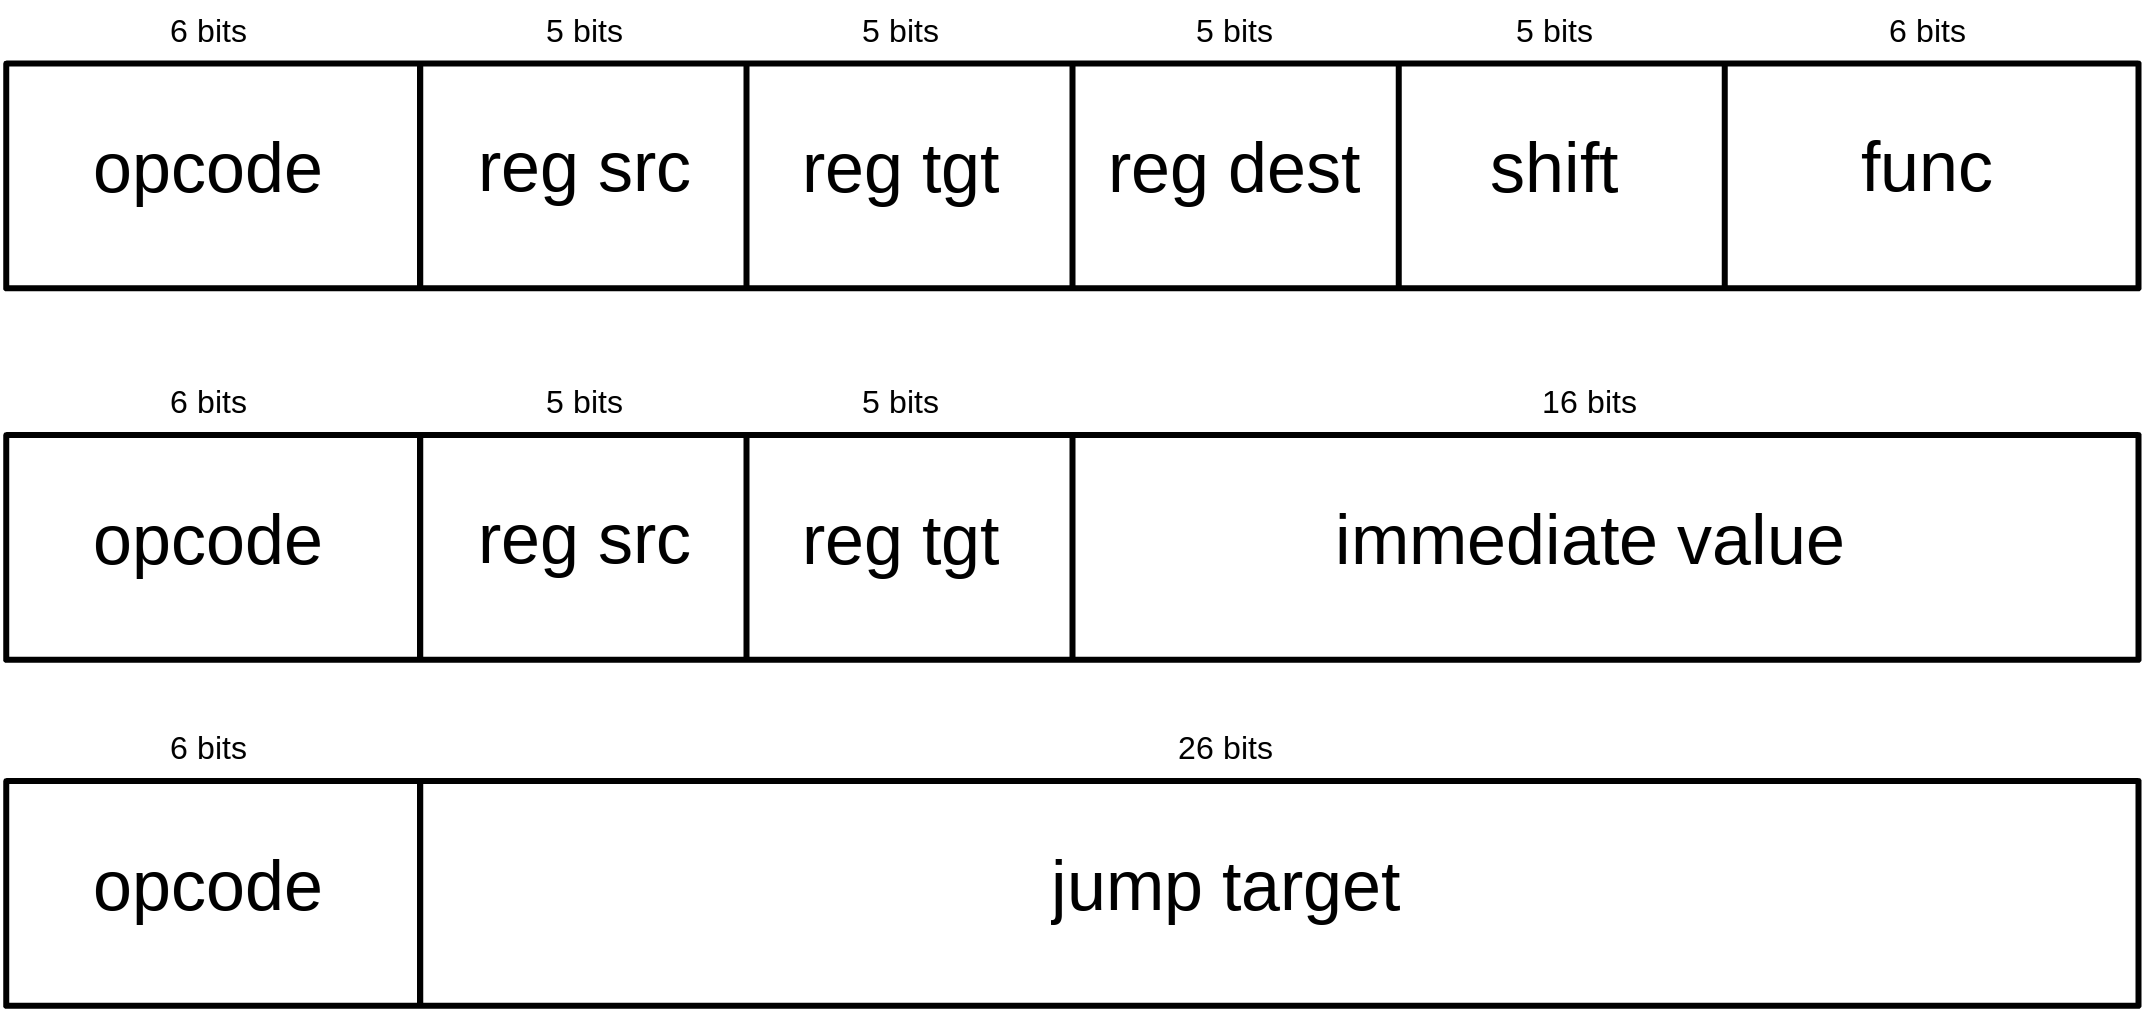
\includegraphics[width=0.8\textwidth]{obrazky-figures/instruction.png}
	\caption[\textit{MIPS I} typy instrukcí]{\textit{MIPS} má celkem 3 způsoby, jak zakódovat instrukci do 32 bitů.}
	\label{instruction}
\end{figure}

Instrukční sada \textit{CPU}, založená na architektuře \textit{MIPS I}, obsahuje relativně malý počet instrukcí. 
Tato sada zahrnuje \textit{40} základních instrukcí a \textit{29} rozšířených instrukcí, což dohromady činí \textbf{69} instrukcí celkem. Mapa instrukcí je podchycena v obrázku \ref{instruction-map}. 
Tyto instrukce jsou navrženy tak, aby každá z nich zabírala jeden procesorový takt, čímž je udržována neustále plněná 5-ti úrovňová linka. 
Díky této filozofii mají instrukce velmi málo zodpovědností a jsou ve své podstatě velmi jednoduché.

Aby se předešlo složitému dekódování instrukcí, jak tomu je například u architektury \textit{x86\_64}, 
kde každá instrukce může mít proměnlivou délku, \textit{MIPS I} definuje každou instrukci jako 32-bitové slovo. 
Horních 6 bitů pak definuje kódování specifické instrukce. Proto lze každou instrukci rozdělit do zhruba tří tříd, viz obrázek \ref{instruction}. \textit{MIPS} Instrukce v emulátoru je implementována jako sjednocení bitových polí. V \textit{C++} lze využít anonymních struktur a sjednocení, kde jednotlivé bitové alokace se mohou překrývat a tedy umožňuje emulátoru snadno instrukce interpretovat.

\subsection{Koprocesory}

\textit{MIPS R3000A} má ve své instrukční sadě podporu pro celkem 4 různé koprocesory, avšak \textit{PlayStation} využívá pouze 2 z nich\footnote{CPU specifikace \cite{PSXSpec}: \url{https://psx-spx.consoledev.net/cpuspecifications/}}. 
Koprocesorové instrukce jsou všestranné a lze za ně substituovat jakýkoliv čip, kromě \textbf{koprocesoru 1}, který je dedikován pro práci s čísly s plovoucí desetinnou čárkou \cite{MIPSInsSpec} (není přítomen v \textit{PlayStation} konzoli).

\subsubsection{Koprocesor 0 - Správce výjimek}

\textbf{Koprocesor 0} slouží ke správě výjimek a přerušení. 
Koprocesor obsahuje nejen informace o typu výjimky nebo o tom, kdo způsobil přerušení, ale také logiku pro zpracování výjimky. 
Procesor při vyhození výjimky uloží současný stav a jeho kontrolní tok je přenesen na rutinu, která se stará o obsluhu výjimky.
Pro správné ukládání stavu při vyhození výjimky je nutné myslet na situaci, kdy se procesor
nachází ve stavu opožděného skoku. Pokud bychom informaci o provedení skoku neuložili při vyhození výjimky,
po zpracování výjimky a obnovení původního stavu procesoru by se původní skok nemusel provést.
To znamená, že při každém procesorovém taktu je nutné ukládat informaci o skokové prodlevě a
zda-li se skok provede.

\subsubsection{Koprocesor 2 - Geometry transformation engine (GTE)}

\textbf{Koprocesor 2} pak zpřístupňuje komponentu \textit{Geometry Transformation Engine (GTE)}, což je hardware specializovaný pro rychlou práci s lineární algebrou. 
Tento koprocesor pracuje se dvěma základními datovými primitivy: 3D vektory (16/32-bitový atom) a 3x3 matice (16-bitový atom). 
Vektory mohou být interpretovány jako body v prostoru nebo jako barvy a pro každý typ má \textit{GTE} dedikované příkazy. 
Funkce \textit{GTE} jsou velmi všestranné, zahrnují rychlé násobení matice s vektorem, normalizaci barev nebo vektoru a interpolaci. 
Tento koprocesor je nepochybně klíčový pro rychlé zpracování geometrie ve hře a efektivnější vykreslení 3D scény.

Hlavní schopností \textit{GTE} je operace implementovaná ve funkci \textit{multiply\_and\_translate}. Tato operace
implementuje násobení 3D matice a 3D vektoru, přičemž výsledek násobení může být také posunut o 3D \textit{translate} vektor. Tyto výpočty jsou dělány čistě na hostovacím \textit{CPU}.

\section{Grafická procesorová jednotka (GPU)}

Grafická jednotka systému je speciálně navržený čip pro hardwarovou podporu rasterizace geometrických primitiv\footnote{GPU specifikace \cite{PSXSpec}: \url{https://psx-spx.consoledev.net/graphicsprocessingunitgpu/}}.
\textit{GPU} pracuje na frekvenci 53.222400 MHz, což znamená, že je o $\frac{11}{7}$ rychlejší než frekvence \textit{CPU}. Všechna komunikace s \textit{GPU} probíhá přes
čtyři registry:

\begin{itemize}
\item{\textbf{GP0} (pouze zápis) - registr pro odesílání rasterizačních příkazů a posílání geometrických dat. Různé grafické příkazy mohou mít různou délku (počet zapsaných 32-bitových slov) a jsou spravovány přes komunikační frontu.}
\item{\textbf{GP1} (pouze zápis) - registr pro modifikaci stavu \textit{GPU} (například: reset, nastavení rasterizačního okna či potvrzení přerušení).}
\item{\textbf{GPUREAD} (pouze čtení) - registr pro čtení \textit{VRAM} paměti nebo pro čtení speciálních registrů.}
\item{\textbf{GPUSTAT} (pouze čtení) - registr pro čtení celkového stavu \textit{GPU}.}
\end{itemize}

\subsection{Video RAM (VRAM)}

\textit{GPU} má také vlastní paměť nazývanou \textit{Video RAM (VRAM)}. Paměť je rozdělena do 512 řádků o 1024 16-bitových slovech.
Celková kapacita paměti \textit{VRAM} tedy činí: $1024 \times 512 \times 2 = 1048576 B = 1 MiB$\footnote{GPU VRAM \cite{PSXSpec}: \url{https://psx-spx.consoledev.net/graphicsprocessingunitgpu/\#gpu-video-memory-vram}}. 

\textit{VRAM} paměť slouží pouze k ukládání textur, palet pro
indexované textury (\textit{CLUT}, viz sekci [\ref{clut}]) a výsledného \textit{framebufferu}. Jakákoli data o kreslených primitivech (pozice vrcholů či texturovacích souřadnicích)
musí být předána přes registr \textbf{GP0} a jsou okamžitě vykreslena a tedy tyto informace \textit{VRAM} nemůže obsahovat. 

\textit{GPU} má potom 2 různé módy interpretace \textit{VRAM framebufferu} týkající se barevné hloubky. Při vykreslování
na obrazovku může být \textit{VRAM} interpretována jako sekvence 16-bitových barev (kde nevýznamnější bit slouží jako maska a zbytek jsou 5-bitové RGB hodnoty), nebo
24-bitových barev (8-bitové RGB hodnoty). Oba módy mají svoje pravidla a omezení. Ačkoliv \textit{GPU} může rasterizovat primitiva v obou módech, obecně
ve většině her platilo, že pokud se renderovala 3D scéna využíval se 16-bitový mód, protože pak ve \textit{VRAM} paměti zbylo více místa pro textury. 24-bitový mód se
pak většinou používal pouze u přehrávání videí, kde se ve \textit{VRAM} paměti nemohlo ukládat v zásadě nic jiného než \textit{framebuffer}, protože 24-bitový \textit{framebuffer} při \textit{dvojitém bufferingu}\footnote{Double-buffering: \linebreak \url{https://en.wikipedia.org/wiki/Multiple_buffering\#Double_buffering_in_computer_graphics}}
mohl zabírat přes polovinu celé \textit{VRAM} paměti (v závislosti na velikosti videa). 

\subsection{Geometrická primitiva}

\textit{GPU} dokáže vykreslit 3 geometrická primitiva:

\begin{itemize}
    \item{Osově zarovnaný obdélník}
    \item{Čára/Polyčára}
    \item{Trojúhelník/Čtyřúhelník}
\end{itemize}

Všechna tato primitiva lze kreslit pomocí \textbf{GP0} registru\footnote{GPU GP0 registr \cite{PSXSpec}: \url{https://psx-spx.consoledev.net/graphicsprocessingunitgpu/\#gpu-other-commands}}, 
přičemž je nutné zapsat správný počet argumentů do tohoto registru na základě prvního 32-bitového slova příkazu.
Počet argumentů daného primitiva závisí především na různých vlastnostech daného primitiva.
Aby emulátor získal korektně všechny argumenty, emulátor v \textit{GPU} interně uchovává příchozí data ve frontě, přičemž
podle daného příkazu očekává určitý počet argumentů. Po provedení \textbf{GP0} příkazu se tato fronta vypláchne a čeká se na další příkaz.
Ačkoliv ne všechny primitiva mohou mít všechny vlastnosti, \textit{GPU} dokáže rasterizovat jednotlivá primitiva následujícími způsoby\footnote{GPU Semi-transparency \cite{PSXSpec}: \url{https://psx-spx.consoledev.net/graphicsprocessingunitgpu/\#semi-transparency}}:\\[\baselineskip]
\begin{minipage}{\textwidth}
\begin{itemize}
\item{\textbf{Texturovací koordináty} - Primitivum má k sobě přiřazenou texturu a každý vrchol má asociované texturovací koordináty.}
\item{\textbf{Průhlednost} - Na základě předchozího obsahu ve \textit{VRAM} paměti dokáže \textit{GPU} mixovat barvy ve čtyřech různých módech:
    \begin{itemize}
        \item{\textit{half-each} => $result = \frac{background + source}{2}$}
        \item{\textit{additive} => $result = background + source$}
        \item{\textit{subtractive} => $result = background - source$}
        \item{\textit{$\frac{additive}{4}$} => $result = background + \frac{source}{4}$}
    \end{itemize}
}
\item{\textbf{Gouraudovo stínování} - Tento atribut je svým názvem trochu zavádějící, neboť gouraudovo stínování v moderní informatice souvisí spíše s výpočtem \textit{per-vertex} osvětlení. V tomto případě jde ovšem pouze o zapnutí interpolace atributů mezi vrcholy primitiva.}
\end{itemize}
\end{minipage}\\[\baselineskip]
Tyto atributy jsou při komunikaci přes \textbf{GP0} registr nashromážděny a použity v emulátoru při rasterizaci primitiva, viz sekci [\ref{primitive-rasterization}].

\subsection{Color Lookup Table (CLUT) vyrovnávací paměť} \label{clut}

V drtivé většině případů, kdy dané geometrické primitivum má asociovanou texturu, pixely této textury jsou indexy do specifické palety barev, neboli \textit{Color Lookup Table (CLUT)}, která je uložena spolu s texturou uvnitř \textit{VRAM}.
Díky tomu mají textury relativně mnohem menší velikost, než kdybychom ukládali texturu s absolutními hodnotami pixelů, což za své doby
bylo bezpodmínečně nutné, protože nakonec \textit{VRAM} má pouze \textit{1 MiB} místa. \textit{CLUT} je spolu s texturou uložena ve \textit{VRAM} jako
lineární sekvence bytů.

Pokud ovšem rasterizujeme kupříkladu texturovaný obdélník, šance, že se \textit{CLUT} bude radikálně měnit je blízko nule. Jelikož každé
čtení z \textit{VRAM} stojí GPU cykly, \textit{GPU} má vyrovnávací paměť speciálně dedikovanou pro \textit{CLUT}, přičemž
jakmile započne rasterizace texturovaného primitiva, \textit{GPU} nejdříve zkontroluje jaký \textit{CLUT} region dané primitivum vyžaduje podle
příslušných \textit{CLUT} koordinátů. Pokud se tyto koordináty odlišují od posledních použitých \textit{CLUT} koordinátů, nebo se liší barevná
hloubka od poslední použité, \textit{CLUT} vyrovnávací paměť se vypláchne a naplní se novými \textit{CLUT} daty.

Při čtení texturových dat se pak exkluzivně používá \textit{CLUT} vyrovnávací paměť. To ovšem platí jen u specifické barevné
hloubky pixelu. \textit{CLUT} vyrovnávací paměť se používá pouze u \textit{4-bitové} a \textit{8-bitové} barevné hloubky. \textit{16-bitová} hloubka
pak indikuje absolutní ukládání barev v textuře bez \textit{CLUT}.

\subsection{Barvy}

Jak bylo zmíněno, \textit{GPU} dokáže pracovat s 24-bitovými barvami, které obsahují 3 základní barevné komponenty (červená, zelená a modrá). 
Každému z těchto komponent je alokováno 8 bitů a dále dokáže pracovat s 15-bitovými barvami, kde každé komponentě je přiřazeno pouze 5 bitů.

Pokud programátor chtěl detaily 24-bitové hloubky, ale nechtěl přepnout \textit{VRAM} do 24-bitového módu a mít tak méně prostoru pro kreslení, \textit{GPU} poskytovalo hardwarovou funkcionalitu přesně pro tyto účely. 
Zatímco 15-bitová barva (plus maskovací bit) se pouze zkopíruje do paměti \textit{VRAM}, 24-bitová barva může být za pomocí techniky \textit{dithering}\footnote{GPU dithering \cite{PSXSpec}: \url{https://psx-spx.consoledev.net/graphicsprocessingunitgpu/\#24bit-rgb-to-15bit-rgb-dithering-enabled-in-texpage-attribute}} rozdistribuována do kreslícího okolí, čímž může ošálit lidské oko a získat tak lepší barevnou hloubku. 

Paměť \textit{VRAM} v 16-bitovém módu v každém fragmentu také ukládá extra 1 bit, který figuruje jako kreslící maska. 
Pokud je nejvyšší bit v 16-bitové barvě nastaven na 1, pak tento fragment bude ignorován a nic se do něj nevykreslí.

\subsection{Rasterizace primitiv} \label{primitive-rasterization}

U každého ze 3 geometrických primitiv, které \textit{GPU} dokáže vykreslit, je nutno zvolit správný algoritmus pro jeho rasterizaci.
U rasterizace osově zarovnaného obdélníku stačí zjistit maximum a minimum ve 2D prostoru. Tento omezený prostor může být následně vyplněn.

Rasterizace čáry vyžaduje sofistikovanější přístup, čímž je \textbf{Digital Differential Analyzer (DDA) algoritmus}\footnote{DDA algoritmus: \newline \url{https://en.wikipedia.org/wiki/Digital_differential_analyzer_(graphics_algorithm)}}, 
který na základě výpočtu sklonu čáry dokáže vyplnit fragmenty mezi dvěma body ve 2D prostoru.
Algoritmus \textit{DDA} zjednodušeně funguje následujícím způsobem:\\[\baselineskip]
\begin{minipage}{\textwidth}
\begin{enumerate}
    \item{spočítáme rozdíl $d = line_{end} - line_{start}$}
    \item{na základě kvadrantu prohodíme $x$ a $y$ souřadnice rozdílu $d$ i souřadnic čáry $line_{start}$ a $line_{end}$}
    \item{vypočítáme sklon čáry jako $k = d.y / d.x$}
    \item{ve smyčce od $line_{start}.x$ do $line_{end}.x$ vyplňujeme pixely, přičemž $y$ souřadnici při každé iteraci navyšujeme o hodnotu $k$}
\end{enumerate}
\end{minipage}\\[\baselineskip]
Pro urychlení algoritmu lze použít \textit{fixed-point} aritmetiku, kde při každé adresaci fragmentu operace pracuje pouze s celými čísly.

Trojúhelníková rasterizace se řadí mezi vyplňovací rasterizační algoritmy. 
Pro jeho implementaci jsem zvolil základní variantu \textbf{Pinedova algoritmu} \cite{PinedaAlgorithm}. 
Jeho podstata závisí na rozdělení jednotlivých hran trojúhelníku na poloroviny a u každého fragmentu zjišťovat jeho 
polohu v závislosti na všech polorovinách daného trojúhelníku.
Zjednodušený algoritmus, který dokáže trojúhelník rasterizovat vypadá zhruba takto:\\[\baselineskip]
\begin{minipage}{\textwidth}
\begin{enumerate}
    \item
    {
        Spočítáme ohraničující obdélník:
        \[ topleft = min(tri_a, tri_b, tri_c) \] 
        \[ bottomright = max(tri_a, tri_b, tri_c) \]
    }
    \item
    {
        Spočítáme jednotlivé hrany trojúhelníku jako vektory: 
        \[ \vec{delta_{ba}} = tri_b - tri_a \] 
        \[ \vec{delta_{cb}} = tri_c - tri_b \] 
        \[ \vec{delta_{ac}} = tri_a - tri_c \]
    }
    \item
    {
        Pro každý fragment ohraničujícího obdélníku zjistíme relativní polohu daného fragmentu 
        vůči třem hraničním polorovinám pomocí 2D vektorového součinu:

        \[ planepos_{cb} = \vec{delta_{cb}} \times \vec{(fragment_{pos} - tri_b)}\]
        \[ planepos_{ac} = \vec{delta_{ac}} \times \vec{(fragment_{pos} - tri_c)}\]
        \[ planepos_{ba} = \vec{delta_{ba}} \times \vec{(fragment_{pos} - tri_a)}\]
    }
    \item
    {
        Znaménka jednotlivých relativních pozicí pak určují, na které straně poloroviny
        se daný fragment nachází. Pokud všechny relativní pozice mají stejné znaménko,
        znamená to, že se fragment vyskytuje uvnitř trojúhelníku:

        \[ sign(planepos_{cb}) = sign(planepos_{ac}) = sign(planepos_{ba}) \]
    }
\end{enumerate}
\end{minipage}\\[\baselineskip]

Ačkoliv tento přístup je správný, kalkulace vektorového součinu pro každý fragment je zbytečná
práce. Místo toho, vektorový součin lze vypočítat pouze pro první fragment, a při každé
změně fragmentu stačí pouze přičíst \textit{delty}. To znamená, že místo 6 násobení a 3 odčítání
pro každou složku fragmentu pro výpočet vektorového součinu, nám stačí pouze 3 sčítání.

Při zpracování trojúhelníku a přiřazování atributů k jednotlivým vrcholům, je nutno
myslet na orientaci trojúhelníku (pořadí vrcholů ve směru/proti směru hodinových ručiček).
Ačkoliv \textit{GPU} pracuje čistě s protisměrném pořadí hodinových ručiček, data
přicházející do \textit{GPU} nejsou nutně v tomto pořadí.

Pokud \textit{GPU} v emulátoru dostane data v opačném pořadí, interně tuto chybu detekuje pomocí
vektorového součinu dvou hran trojúhelníku. Na základně znaménka poté jednotlivé
vrcholy prohodí pro správné protisměrné pořadí hodinových ručiček.

U rasterizace čáry/polyčáry a trojúhelníku, rasterizace reálného \textit{GPU} využívá
\textit{fixed-point} aritmetiky, což má za následek, že vykreslené polygony mají tendenci
se "chvět", protože jakmile jsou polygony transformovány pomocí \textit{GTE}, výsledné
vrcholy mají celočíselné koordináty. Bohužel existují konfliktní informace o tom,
kolik bitů je alokováno pro celočíselnou část a kolik pro zlomkovou část a ve které
části rasterizace se bere pouze celočíselná část koordinátu. V tomto bodě byla nutná
experimentace, přičemž nejvěrohodnější výsledky byly dosaženy s 32-bitovou \textit{fixed-point}
hodnotou s 12-bitovou zlomkovou částí.

\subsection{Zvýšení rozlišení}

Zvýšení rozlišení se týká především \textit{GPU} a rasterizace jednotlivých primitiv. 
\textit{GPU} ve svém interním stavu ukládá mimo jiné meze \textit{framebufferu}. 
Tyto meze pak figurují při rasterizaci, kde jakýkoliv pokus kreslit mimo tyto meze bude ignorován. 
Zároveň tyto meze určují, odkud ve \textit{VRAM} paměti se budou brát data pro zasílání 
do \textit{CRT} monitoru.

Pro tyto účely je nutné spravovat separátní \textit{High resolution VRAM} (\textit{Hi-res VRAM}) paměť, která podle nastavení 
bude mít násobek velikosti současné reálné \textit{VRAM} paměti uvnitř \textit{GPU}.

U rasterizaci primitiv je pak nutné zachytit a správně přepočítat jejich pozice, stejně jako 
upravit jejich omezující vlastnosti. Největší potíž však je při adresaci textur a jejich palet. 
Při každém zápisu textury a indexu barvy je nutné koordináty přemapovat o současný násobek velikosti \textit{Hi-res VRAM}. Tento problém je vyřešen tak, že při používání \textit{Hi-res VRAM} kdykoliv rasterizace vyžaduje barvu textury, rasterizér sáhne do původní \textit{VRAM} a výsledek je rozdistribuován do okolí \textit{Hi-res VRAM}. 
To znamená, že při vykreslování ve vyšším rozlišení se musí kreslit do obou \textit{VRAM} i \textit{Hi-res VRAM} současně.

\section{Jednotka přímého přístupu do paměti (DMA)}

Jelikož \textit{CPU} má hodinovou rychlost 33.8688 MHz, jakýkoliv přenos dat je nesmírně pomalý. 
Tento fakt je pouze umocněn v situaci, kdy program chce přenést data z paměti \textit{RAM} do jiné hardwarové komponenty. 
Pokud bychom měli jednoduchou smyčku pro kopírování dat s prokládanou inkrementací indexu do paměti (abychom vyplnili zpoždění čtení z paměti \textit{RAM} popsané v sekci [\ref{load-delay}]),
dostaneme 4 instrukce pro kopírování a 3 instrukce pro správu cyklu, viz obrázek \ref{slow-copy}.

\begin{figure}[hbt]
	\centering
	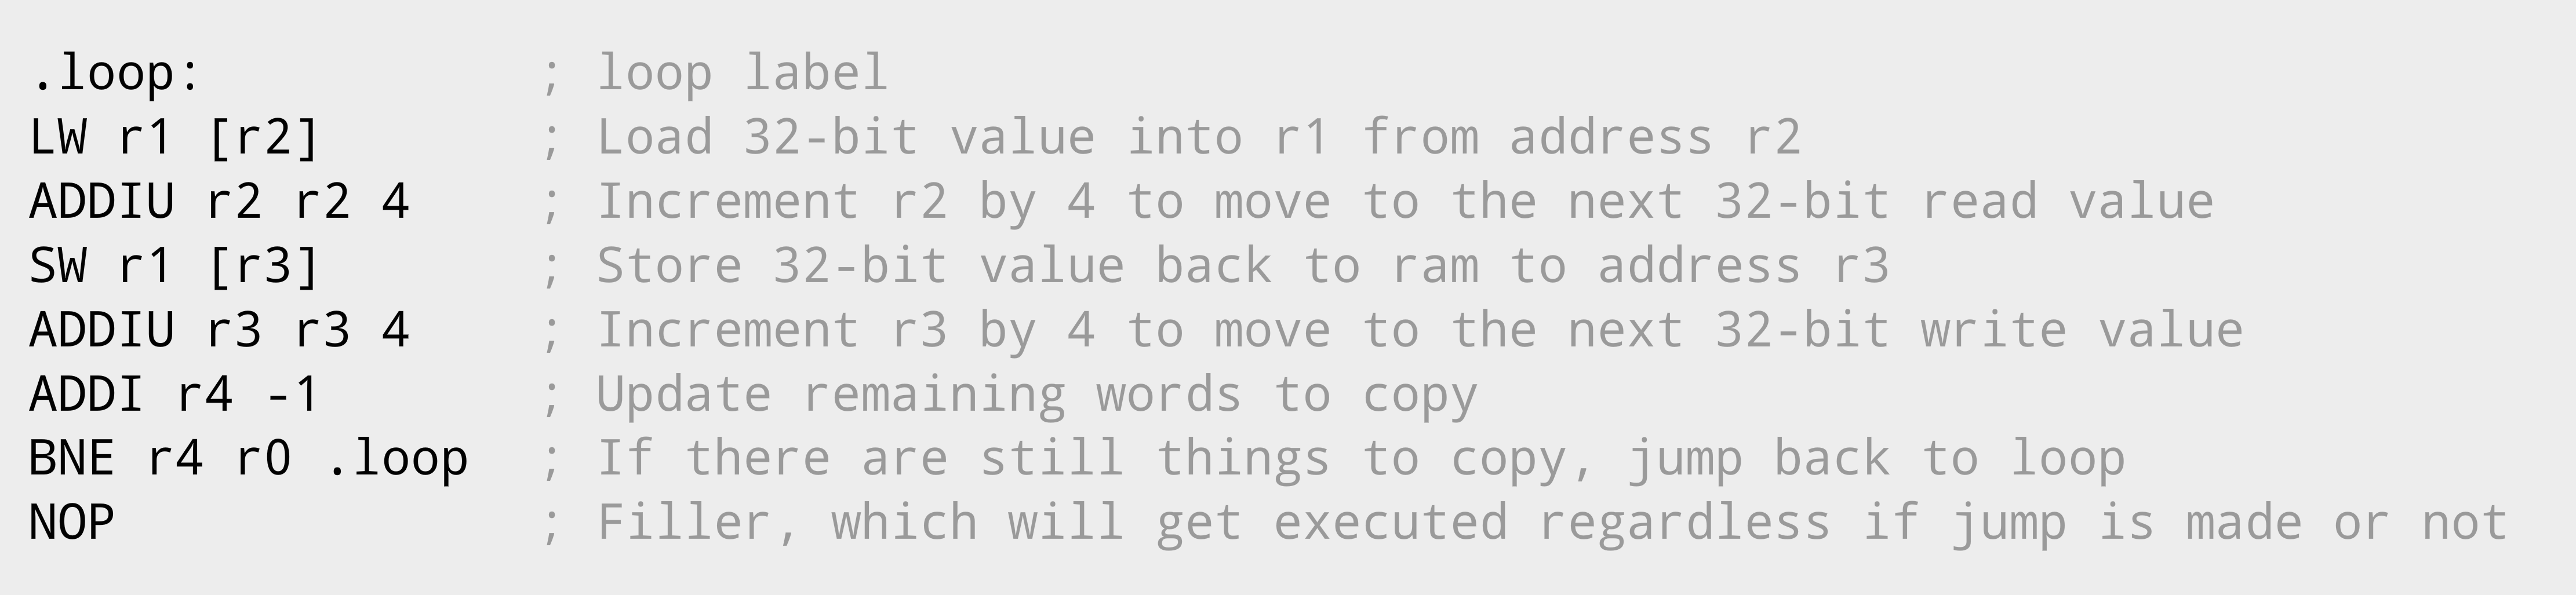
\includegraphics[width=1.0\textwidth]{obrazky-figures/slow-copy.png}
	\caption[\textit{CPU} program pro přesouvání dat bez \textit{DMA}]{Pomocí 7 instrukcí a správným prokládáním lze docílit maximální rychlosti při kopírování dat. Každý cyklus přenese 4 byty.}
	\label{slow-copy}
\end{figure}

Z teoretického hlediska to znamená, že ideální rychlost přenosu činí $\frac{33.8688}{4+3}\times4 = 19.3536 MB/s$. 
Kvůli této nevýhodě obsahuje \textit{PlayStation} komponentu \textit{Direct Memory Access (DMA)}, 
která slouží výhradně k~velmi rychlému přenosu dat mezi pamětí \textit{RAM} a hardwarovými komponentami. 
\textit{DMA} má celkem 7 různých kanálů, přičemž každý kanál specifikuje komunikující komponenty\footnote{DMA \cite{PSXSpec}: \url{https://psx-spx.consoledev.net/dmachannels/}}.\\[\baselineskip]
\begin{minipage}{\textwidth}
\begin{itemize}
    \item{\textbf{DMA Kanál 0. - MDECIN} - Z \textit{RAM} do \textit{MDEC} vstupu}
    \item{\textbf{DMA Kanál 1. - MDECOUT} - Z \textit{MDEC} výstupu do \textit{RAM}}
    \item{\textbf{DMA Kanál 2. - GPU} - Mezi \textit{RAM} a \textit{GPU}}
    \item{\textbf{DMA Kanál 3. - CDROM} - Z \textit{CD-ROM} do \textit{RAM}}
    \item{\textbf{DMA Kanál 4. - SPU} - Mezi \textit{RAM} a \textit{SPU}}
    \item{\textbf{DMA Kanál 5. - PIO} - Mezi \textit{RAM} a \textit{Expansion Port}}
    \item{\textbf{DMA Kanál 6. - OTC} - Mezi \textit{RAM} a \textit{GPU Ordering Table}}
\end{itemize}
\end{minipage}
\\[\baselineskip]
\textit{DMA} také poskytuje celkem 3 různé módy přenosu:\\[\baselineskip]
\begin{minipage}{\textwidth}
\begin{itemize}
    \item{\textbf{Word Copy} - Jde o rychlý přenos lineární sekvence 32-bitových hodnot. Maximálně se může přenést až \textit{65536} 32-bitových hodnot.}
    \item{\textbf{Block Copy} - Přenáší se bloky o uživatelem definované délce. Po dokončení přenosu jednoho bloku se pak čeká na připravenosti specifikované komponenty. Tento mód se především používá při přenosu dat z a do \textit{MDEC} komponenty. }
    \item{\textbf{Linked List Copy} - Přenášená data se dělí na hlavičku a tělo. Hlavička obsahuje délku těla a adresu další hlavičky. Celá datová struktura je pak řetězec hlaviček a těl. Tento mód je hlavně využit při zasílání renderovacích příkazů do \textit{GPU}. }
\end{itemize}
\end{minipage}
\\[\baselineskip]

Každý mód přenosu poskytuje velmi rychlé přenosy, protože \textit{DMA} využívá \textit{DRAM Hyper Page} mód, 
což umožňuje \textit{DMA} přistupovat k \textit{DRAM} řádkům v zásadě v jednom procesorovém cyklu. 
Tento přístup má minimální režii, která způsobí, že pro každých 17 cyklů se přečte 16 32-bitových slov. To znamená, že teoretické maximum přenosové rychlosti činí ${33.8688}\times4\times\frac{16}{17} = 127.5060 MB/s$.

Při \textit{DMA} přenosu má \textit{CPU} přísná pravidla ohledně přístupu do paměti. 
Pokud probíhá přenos, \textit{CPU} může přistupovat k vyrovnávacím pamětem a ke svým dvěma koprocesorům. 
Jakmile se \textit{CPU} pokusí přistoupit do paměti, je jeho chod pozastaven, dokud \textit{DMA} přenos není dokončen.

Díky tomuto faktu lze v emulátoru jakoukoliv \textit{DMA} synchronizaci obejít tím, že se celý přenos provede najednou a \textit{CPU} je pozastaveno. 
Výjimkou je \textit{MDEC}, kde pro simulaci synchronizace tato komponenta obsahuje speciální příznak, který je modifikován při začátku, či při dokončení dekódování,
a který indikuje připravenost přenosu dat z a do \textit{MDEC} komponenty.

\textit{DMA} umožňuje pomocí speciálního registru definovat priority jednotlivých kanálů.
To znamená, že se některé \textit{DMA} kanály dostanou ke slovu dříve než ostatní. Toto chování
je v emulátoru implementováno pomocí prioritní fronty (\textit{priority\_queue} z \textit{C++} standardní knihovny). 
Při každém emulačním kvantu \textit{DMA} ovladač extrahuje jednotlivé priority a zkonstruuje
prioritní frontu, pomocí níž jsou jednotlivé kanály zpracované ve správném pořadí. 


\section{Ovladač přerušení/výjimek}

Aby \textit{CPU} mělo přehled o různých událostech, jako je například dokončení \textit{DMA} přenosu, 
\textit{PlayStation} má 2 úzce svázané hardwarové komponenty: \textit{Ovladač přerušení} a \textit{Ovladač výjimek}. 
\textit{Ovladač přerušení} je propojen v podstatě se všemi ostatními komponentami, od kterých je schopen přijímat požadavky na přerušení. 
Tento čip také obsahuje stavový registr, ze kterého lze zjistit kdo přerušení způsobil.

To ale není dostatečné pro pozastavení chodu procesoru. 
\textit{Ovladač přerušení} je napojen na \textit{koprocesor 0 CPU}, tedy \textit{Ovladač výjimek}, 
přičemž přerušení je pouze zvláštní typ výjimky.

\textit{BIOS} následně disponuje předem definovanými vektory adres, na jejichž základě se rozhoduje 
kam přesměrovat řízení procesoru a následně zpracovat výjimku.

\section{Časovače}

\textit{PlayStation} má 3 různé druhy časových zdrojů, plus jeden časový zdroj pro \textit{CPU}. 
Jelikož se tyto 3 hardwarové složky příliš neliší, v emulátoru jsem využil \textit{STL} knihovnu \textit{C++} k instanciaci každého ze tří zdrojů.

\textit{První} zdroj se nazývá \textbf{Dot Clock}. Tento zdroj souvisí s renderovacím módem \textit{GPU} komponenty. 
\textit{Dot} v tomto kontextu reprezentuje jeden vykreslený fragment (tzn. ne pixel na obrazovce. Fragment může mít větší či menší velikost než pixel.) a tento 
zdroj tedy počítá počet vykreslených fragmentů, přičemž rychlost závisí na vertikálním rozlišení \textit{GPU}.

\textit{Druhý} zdroj také souvisí s \textit{GPU} a jeho název je \textbf{Horizontal Blank Clock}. 
Pokaždé, když \textit{GPU} dokončí kreslení jednoho řádku \textit{Framebufferu}, tento zdroj je inkrementován o jedničku. 
Rychlost závisí na regionu konzole a verzi \textit{BIOSu} (\textit{NTSC}/\textit{PAL}).

\textit{Třetí} zdroj je \textbf{System Clock}, který odráží zdroj hodin \textit{CPU}, přičemž je ale podělen osmi.
Každý z těchto časovačů má také schopnost vyvolat přerušení, pokud dosáhne určité hodnoty. 
Všechny tyto časovače kromě svých specifických zdrojů mají také zdroj hodin \textit{CPU} a jsou schopny svůj zdroj měnit\footnote{Časovače \cite{PSXSpec}: \url{https://psx-spx.consoledev.net/timers/}}.
Časovače pak ve hrách byly využívány pro různé účely, jako například:

\begin{itemize}
    \item{Semínko pro generátor náhodných čísel}
    \item{Speciální (per-scanline) vizuální efekty}
\end{itemize}

\section{Dekodér makrobloku (MDEC)}

Tento hardwarový čip je jedním z hlavních komponent, která učinila \textit{PlayStation} velmi populární konzolí.
Jelikož se \textit{Sony} rozhodlo použít \textit{CD} jako hlavní úložiště pro hry, každá hra měla na tu dobu
velký prostor. V porovnání se svým konkurentem, \textit{Nintendo 64}, který mohl ukládat maximálně \textit{64 MB},
\textit{PlayStation} disponoval až \textit{600 MB}, přičemž hra mohla obsahovat i více disků a hráč mohl během hry
měnit disky podle postupu ve hře.

Takový prostor bylo třeba využít a \textit{Sony} se rozhodlo pro full-motion video. \textit{MDEC} je čip speciálně věnovaný
na dekódování patentovaného formátu videa. Hlavní myšlenkou tohoto formátu byla \textit{JPEG} komprese obrázku. \textit{JPEG} používá
několik kompresních technik, které efektivně kombinuje dohromady. Obrázek je rozdělen na \textit{makrobloky} o velikosti
8x8 nebo 16x16 pixelů. Tyto bloky jsou následně převedeny do \textit{YCbCr} barevného formátu a \textit{CbCr} složky jsou
zploštěny na polovinu, přičemž složka intenzity \textit{Y} je zachována v plném rozlišení. 
Toto je možné, protože lidské oko je citlivější na intenzitu světla než na samotnou diferenci barev, aby člověk ve tmě byl schopen
alespoň rozlišit tvary.
Poté je provedena \textit{Discrete Cosine Transform (DCT)}, frekvenční analýza a přebytečné frekvence jsou odstraněny
pomocí kvantizační tabulky. Výsledný makroblok je přeorganizován \textit{Zig Zag} vzorem, aby potom následující technika \textit{Run-Length}
byla schopna zakódovat daný makroblok co nejefektivněji. \textit{JPEG} pak využívá \textit{Huffmanova} kódování pro vytvoření výsledného datového toku.
Dekódování probíhá velmi podobným způsobem, ale obráceným směrem, viz obrázek \ref{mdec-decoding}\footnote{MDEC \cite{PSXSpec}: \url{https://psx-spx.consoledev.net/macroblockdecodermdec/}}.

Formát snímku videa v \textit{PlayStationu} je velice podobný \textit{JPEGu}, s výjimkou toho, že \textit{PlayStation} nepoužívá \textit{Huffmanovo} kódování.
To má za následek mnohonásobně rychlejší dekódování videa, ale samozřejmě uložený video soubor má pak mnohonásobně větší velikost.

\begin{figure}[hbt]
	\centering
	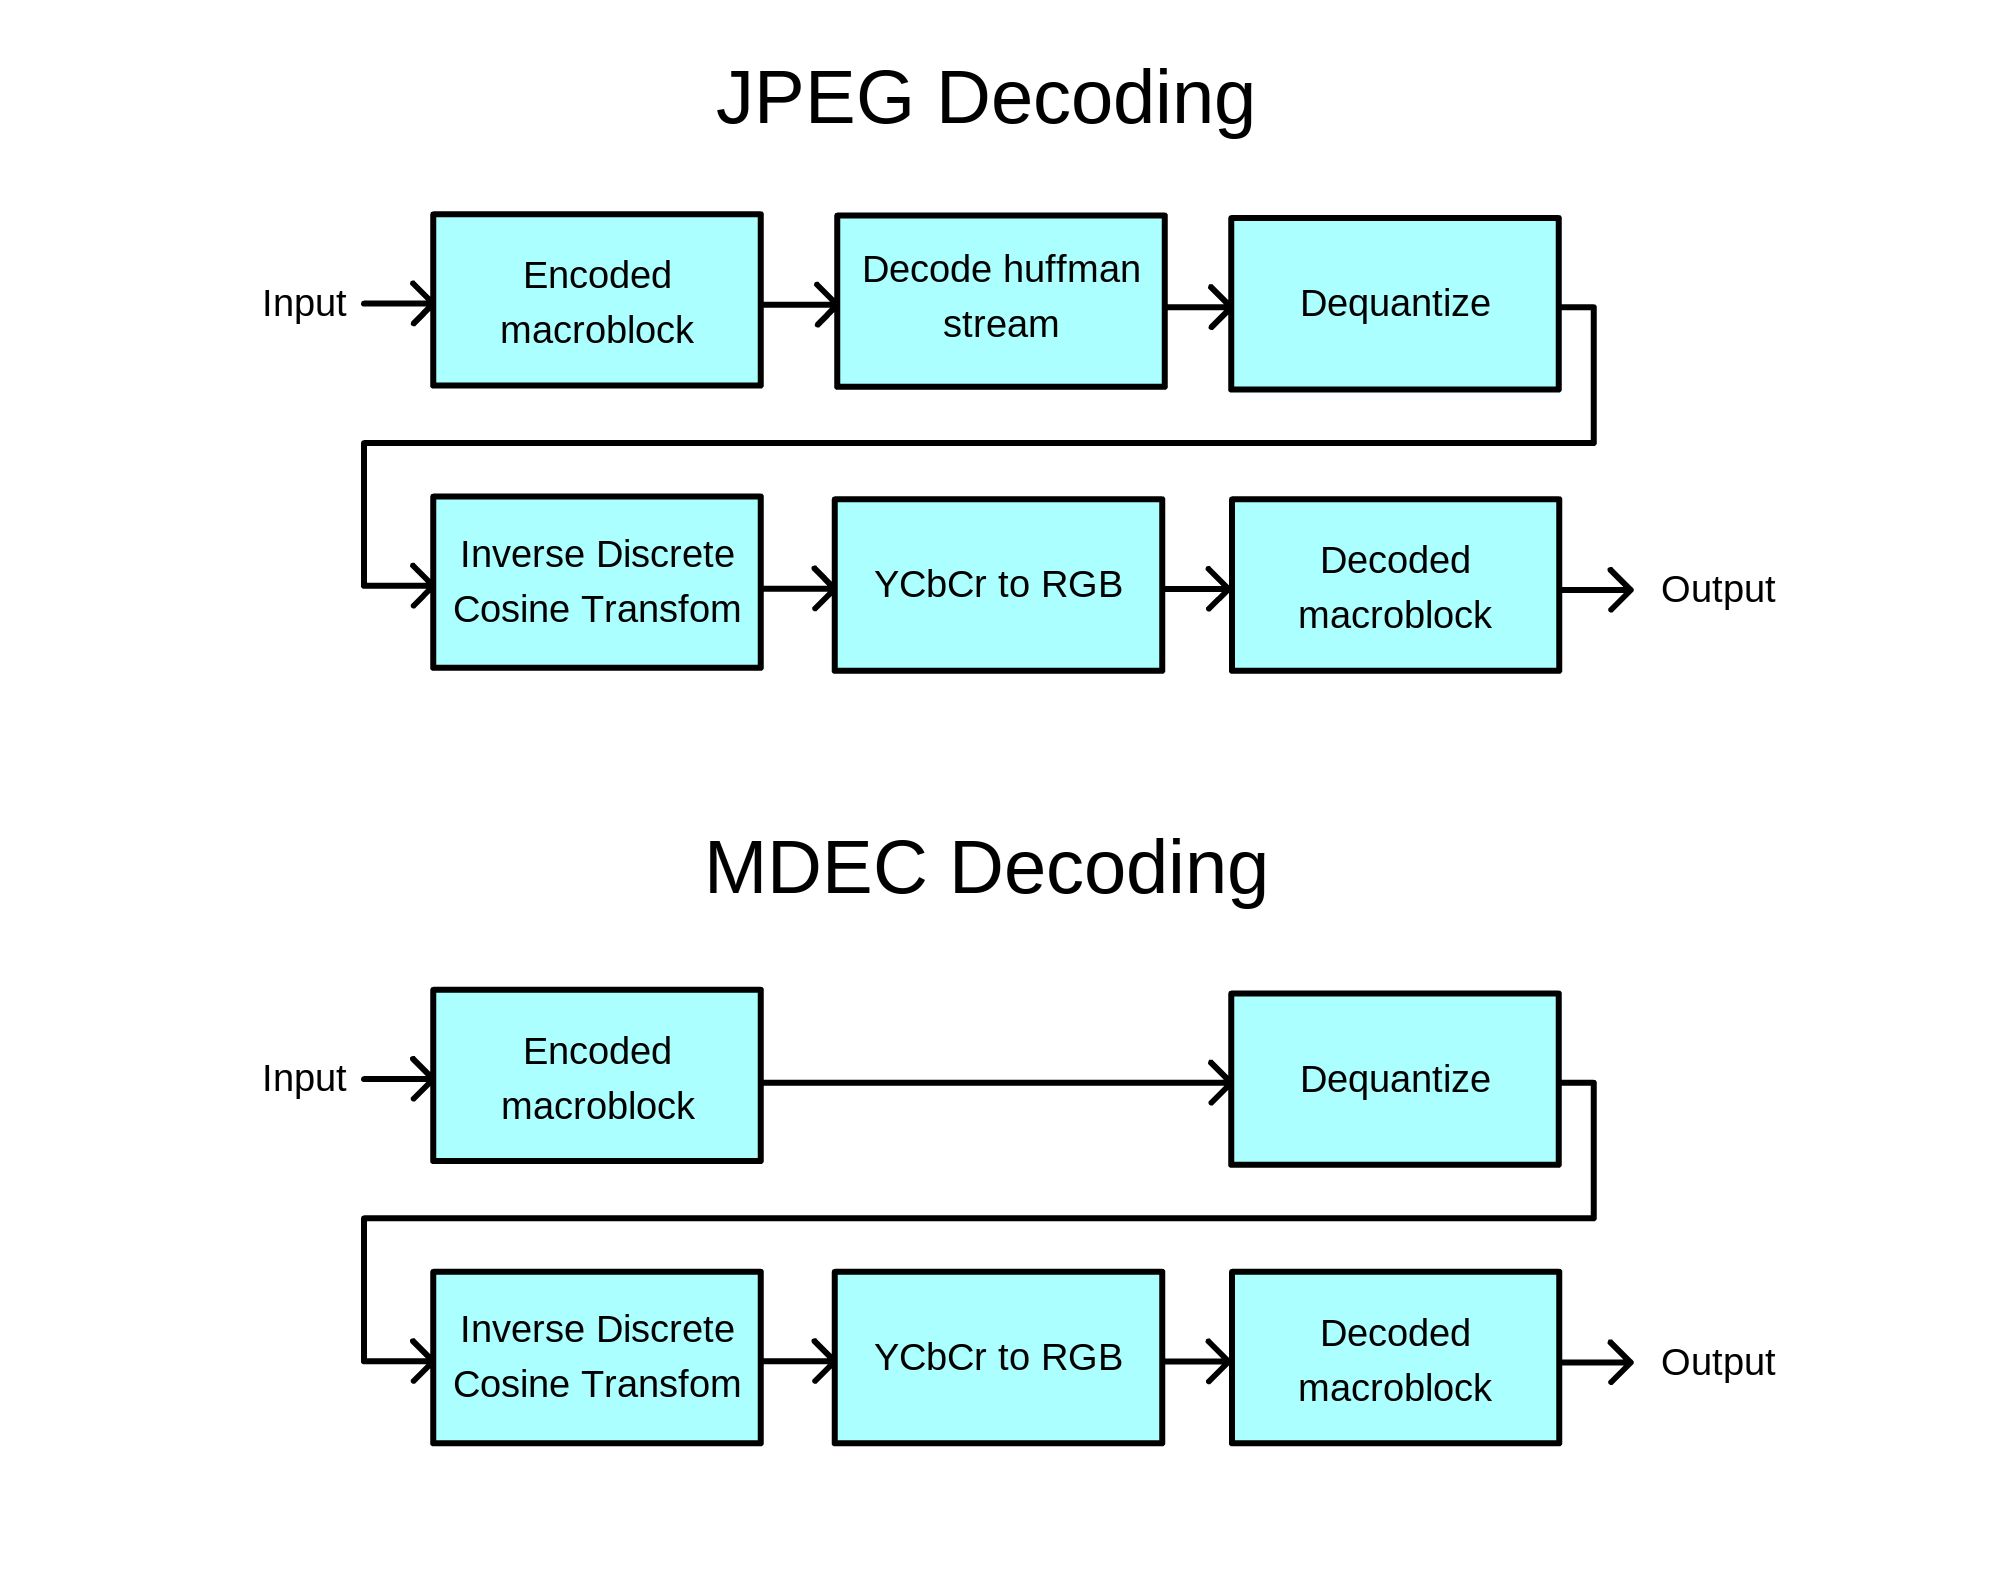
\includegraphics[width=1.0\textwidth]{obrazky-figures/mdec-decoding.png}
	\caption[\textit{MDEC} / \textit{JPEG} dekódování]{\textit{MDEC} má velmi podobnou strukturu jako \textit{JPEG} až na vynechaný krok Huffmanova dekódování.}
	\label{mdec-decoding}
\end{figure}

Při přesunu dat, \textit{MDEC} má speciální příznak pomocí kterého indikuje stav dekódování (připravenost vstupu a výstupu).



\section{CD-ROM mechanika}

\textit{Sony} se rozhodlo použít pro herní úložiště \textit{Compact Disc Extended Architecture (CD-XA)} a standard ISO 9660.
\textit{BIOS} je zodpovědný za analýzu ISO 9660 souborového systému a poskytuje hrám k jednotlivým souborům přístup, čili emulátor se o tuto část
nemusí starat.

\textit{CPU} může komunikovat s \textit{CD-ROM} mechanikou jednak přes registry a příkazy, ale navíc \textit{CD-ROM} má také tři datové fronty,
pomocí nichž se přenášejí data a dotazy na přerušení. Interně \textit{CD-ROM} disponuje celkem \textit{37} příkazy, pomocí kterých
lze manipulovat se čtecím motorem.

Pro správný přístup k \textit{CD} je nutné správně adresovat toto médium. Jelikož je \textit{CD-ROM} spíše chápán jako
úložiště pro audio či video média, disk je adresován pomocí stop. Každá stopa se dá reprezentovat indexem
nebo formátem \textit{minuty (MM):sekundy (SS):zlomky (FF)}. Každý disk má maximálně \textit{74} minut, přičemž v každé minutě
je \textit{60} sekund a každá sekunda obsahuje \textit{75} zlomků. S touto znalostí se pak tento 
formát dá převést na \textit{Logical Block Addressing (LBA)}, což je schopnost adresovat \textit{CD} jako lineární sekvenci bytů.

Hry také měly možnost být prodávány ne na jednom, ale na několika discích. \textit{CD-ROM} má pak schopnost výměny disku
bez resetování konzole. Pomocí vypnutí motoru lze \textit{CD-ROM} mechaniku pozastavit, otevřít poklop, vyměnit disk
a program po uzavření poklopu může bezproblémově pokračovat\footnote{CD-ROM mechanika \cite{PSXSpec}: \url{https://psx-spx.consoledev.net/cdromdrive/}}. Tato funkcionalita ovšem bohužel není v emulátoru implementována a tedy některé hry uživatel nemá schopnost dokončit.

\section{Periférie}

Ačkoliv samotná konzole má vnitřně několik typů periférií, jako jsou I/O a debugovací porty, veřejně dostupná verze konzole má celkem 4 porty, 
se kterými běžný uživatel může interagovat. Z těchto portů slouží 2 na vsunutí \textit{MemoryCard}, 
což figurovalo jako malé úložiště pro uchování postupu ve hrách. 
Zbývající 2 porty pak fungují jako vstupy pro herní ovladače, přičemž existují celkem 3 oficiálně podporované typy: \textit{Digital}, \textit{Analog} a \textit{Mouse}.

Hry mohou individuálně číst z těchto portů a umožňují tak uživateli s konzolí interagovat. 
Veškerá komunikace mezi \textit{CPU} a perifériemi probíhá pomocí \textit{Serial I/O (SIO)}\footnote{Ovladače a paměťové karty \cite{PSXSpec}: \url{https://psx-spx.consoledev.net/controllersandmemorycards/}}.
\textit{PlayStation} měl podporu pro nemálo typů herních ovladačů\footnote{List podporovaných ovladačů \cite{PSXSpec}: \url{https://psx-spx.consoledev.net/controllersandmemorycards/}}, 
ovšem drtivá většina her z \textit{PlayStation} knihovny dokázala používat pouze standardní digitální ovladač.
Čili v emulátoru je implementovaná komunikace pouze pro tento typ ovladače.

Ovladač je v emulátoru implementován jako jednoduchý automat, obsahující stavovou proměnou, která udává, ve které části komunikace se ovladač s \textit{BIOSem} nachází. Na základě
předem určené výměně bytové sekvence\footnote{Komunikace s ovladačem \cite{PSXSpec}: \url{https://psx-spx.consoledev.net/controllersandmemorycards/\#controllers-communication-sequence}} si \textit{CPU} a ovladač vymění synchronizační data, přičemž se na konci této komunikační sekvence předají stavy jednotlivých tlačítek.

\section{Zvuková procesorová jednotka (SPU)}

Zvuková část \textit{PlayStation} systému je relativně nejsložitější hardwarová komponenta. Bohužel, tuto komponentu jsem nebyl schopen přivést
do funkčního stavu. I přesto emulátor musí do jisté míry, alespoň částečně, tuto komponentu simulovat.

\subsection{Zvuková RAM (SRAM)}

Zvukový čip není pouze zodpovědný za zpracování vzorkovaného signálu, ale je také schopen vzorky generovat nebo nad tokem vzorků aplikovat
speciální efekty. Některé zvukové efekty, jako například ozvěna, ovšem vyžadují paměťový prostor. Pro implementaci ozvěny je nutno si pamatovat
předchozí zvukové vzorky, a proto \textit{SPU} má samostatnou paměť \textit{Sound RAM} (\textit{SRAM}). Tato paměť má kapacitu \textit{512KB}, a je zpřístupněna pouze
přes registry \textit{SPU}.

Pro zprovoznění některých her, implementace této paměti byla bezpodmínečně nutná, neboť určité přenosy do \textit{SRAM} paměti se provádí přes
\textit{DMA}. To znamená, že některé hry čekají na přerušení indikující dokončení přenosu, a pokud toto přerušení nepřijde, logika hry se zasekne.

\subsection{Voice}

\textit{SPU} má celkem \textit{24 Voice} kanálů.
\textit{Voice} v tomto kontextu funguje přibližně jako hudební nástroj v \textit{midi} formátu. Do jednotlivého \textit{Voice} kanálu
lze nahrát vzorek hudebního nástroje a poté mu nastavovat výšku tónu. Díky tomu se ušetří
nemálo prostoru, protože hudbu lze pak ukládat jako noty spolu s krátkým vzorkem jednotlivých hudebních nástrojů.
\textit{Voice} také má schopnost generovat pseudo-náhodný šum, což je užitečné například při generování zvuku bubnů, místo toho aby
byl uložen jako tok \textit{ADPCM} vzorků.

\subsection{ADPCM}

Obzvlášť při přehrávání full-motion videa, \textit{Voice} nemusí mít dostatečnou flexibilitu, pro reprodukci
dostatečně detailní zvukové stopy. Pro tyto účely \textit{SPU} poskytuje dekódování a dekompresi \textit{Adaptive differential pulse-code modulation (ADPCM)}\footnote{ADPCM: \url{https://en.wikipedia.org/wiki/Adaptive_differential_pulse-code_modulation}}.